\documentclass[11pt,a4paper]{article}
%%%%%%%%%%%%%%%%%%%%%%%%% Credit %%%%%%%%%%%%%%%%%%%%%%%%

% template ini dibuat oleh martin.manullang@if.itera.ac.id untuk dipergunakan oleh seluruh sivitas akademik itera.

%%%%%%%%%%%%%%%%%%%%%%%%% PACKAGE starts HERE %%%%%%%%%%%%%%%%%%%%%%%%
\usepackage{lmodern}
\usepackage{graphicx}
\usepackage{caption}
\usepackage{microtype}
\captionsetup[figure]{name=Gambar}
\usepackage{tabulary}
\usepackage{minted}
\usepackage{float}
% \usepackage{amsmath}
\usepackage{fancyhdr}
% \usepackage{amssymb}
% \usepackage{amsthm}
\usepackage{placeins}
% \usepackage{amsfonts}
\usepackage[all]{xy}
\usepackage{tikz}
\usepackage{verbatim}
\usepackage[left=2cm,right=2cm,top=3cm,bottom=2.5cm]{geometry}
\usepackage{hyperref}
\hypersetup{
    colorlinks,
    linkcolor={red!50!black},
    citecolor={blue!50!black},
    urlcolor={blue!80!black}
}
\usepackage{subcaption}
\usepackage{multirow}
\usepackage{psfrag}
\usepackage[T1]{fontenc}
\usepackage[scaled]{beramono}
% Enable inserting code into the document
\usepackage{listings}
\usepackage{chngcntr}
\usepackage{xcolor} 
% custom color & style for listing
\definecolor{codegreen}{rgb}{0,0.6,0}
\definecolor{codegray}{rgb}{0.5,0.5,0.5}
\definecolor{codepurple}{rgb}{0.58,0,0.82}
\definecolor{backcolour}{rgb}{0.95,0.95,0.92}
\definecolor{LightGray}{gray}{0.9}
\lstdefinestyle{mystyle}{
	backgroundcolor=\color{backcolour},   
	commentstyle=\color{green},
	keywordstyle=\color{codegreen},
	numberstyle=\tiny\color{codegray},
	stringstyle=\color{codepurple},
	basicstyle=\ttfamily\footnotesize,
	breakatwhitespace=false,         
	breaklines=true,                 
	captionpos=b,                    
	keepspaces=true,                 
	numbers=left,                    
	numbersep=5pt,                  
	showspaces=false,                
	showstringspaces=false,
	showtabs=false,                  
	tabsize=2
}
\lstset{style=mystyle}
\renewcommand{\lstlistingname}{Kode}
%%%%%%%%%%%%%%%%%%%%%%%%% PACKAGE ends HERE %%%%%%%%%%%%%%%%%%%%%%%%


%%%%%%%%%%%%%%%%%%%%%%%%% Data Diri %%%%%%%%%%%%%%%%%%%%%%%%
\newcommand{\studentA}{\textbf{Made Redy Wijaya (121140157)}}
\newcommand{\studentB}{\textbf{Farhan Apri Kesuma (121140179)}}
\newcommand{\studentC}{\textbf{Carlos Piero Parhusip (121140193)}}
\newcommand{\course}{\textbf{Sistem/Teknologi Multimedia (IF4021)}}
\newcommand{\assignment}{\textbf{Tugas Besar}}
\newcommand{\tanggal}{\textbf{11-22-2024}}

%%%%%%%%%%%%%%%%%%% using theorem style %%%%%%%%%%%%%%%%%%%%
\newtheorem{thm}{Theorem}
\newtheorem{lem}[thm]{Lemma}
\newtheorem{defn}[thm]{Definition}
\newtheorem{exa}[thm]{Example}
\newtheorem{rem}[thm]{Remark}
\newtheorem{coro}[thm]{Corollary}
\newtheorem{quest}{Question}[section]
%%%%%%%%%%%%%%%%%%%%%%%%%%%%%%%%%%%%%%%%
\usepackage{lipsum}%% a garbage package you don't need except to create examples.
\usepackage{fancyhdr}
\pagestyle{fancy}
\lhead{\small Made Redy Wijaya (121140157), Farhan Apri Kesuma (121140179), Carlos Piero Parhusip (121140193)}
\rhead{ \thepage}
\cfoot{\textbf{Hand Sign Calculator Menggunakan MediaPipe dan OpenCV}}
\renewcommand{\headrulewidth}{0.4pt}
\renewcommand{\footrulewidth}{0.4pt}

%%%%%%%%%%%%%%  Shortcut for usual set of numbers  %%%%%%%%%%%

\newcommand{\N}{\mathbb{N}}
\newcommand{\Z}{\mathbb{Z}}
\newcommand{\Q}{\mathbb{Q}}
\newcommand{\R}{\mathbb{R}}
\newcommand{\C}{\mathbb{C}}
\setlength\headheight{14pt}

%%%%%%%%%%%%%%%%%%%%%%%%%%%%%%%%%%%%%%%%%%%%%%%%%%%%%%%555
\begin{document}
\thispagestyle{empty}
\begin{center}
	
\includegraphics[scale = 0.15]{Figure/ifitera-header.png}
	\vspace{0.1cm}
\end{center}
\noindent
\rule{17cm}{0.2cm}\\[0.3cm]
Anggota 1: \studentA \hfill Tugas Ke: \assignment\\[0.1cm]
Anggota 2: \studentB \hfill Tanggal: \tanggal\\[0.1cm]
Anggota 3: \studentC \\[0.1cm]
Mata Kuliah: \course \\[0.1cm]
\rule{17cm}{0.05cm}
\vspace{0.1cm}

%%%%%%%%%%%%%%%%%%%%%%%%%%%%%%%%%%%%%%%%%%%%% BODY DOCUMENT %%%%%%%%%%%%%%%%%%%%%%%%%%%%%%%%%%%%%%%%%%%%%


\section*{Hand Sign Calculator Menggunakan MediaPipe dan OpenCV}

\counterwithin{lstlisting}{section}
\counterwithin{figure}{section}
\counterwithin{table}{section}

\section{Pendahuluan}
Interaksi manusia-komputer (Human-Computer Interaction/HCI) terus berkembang, termasuk dalam teknologi berbasis gesture recognition yang memungkinkan perangkat lunak mengenali gerakan tangan sebagai input untuk menjalankan fungsi tertentu \cite{10522212}. Teknologi ini telah banyak diterapkan, salah satunya pada filter Instagram, di mana gesture tangan digunakan untuk memicu efek tertentu secara interaktif. Dalam konteks ini, proyek bertujuan untuk mengembangkan kalkulator berbasis gesture tangan yang terinspirasi dari interaktivitas filter Instagram. Pengguna dapat menggunakan simbol tangan untuk memasukkan angka dan memilih operasi matematika seperti penjumlahan, pengurangan, perkalian, dan pembagian. Teknologi utama yang digunakan meliputi MediaPipe untuk mendeteksi tangan dan OpenCV untuk pemrosesan citra serta antarmuka pengguna. Penelitian ini berfokus pada bagaimana mendeteksi simbol angka berdasarkan pose tangan dan mengintegrasikan hasil deteksi gesture tangan dengan operasi matematika secara real-time \cite{10001800}. Tujuan utama adalah menciptakan kalkulator interaktif yang memanfaatkan teknologi gesture recognition seperti pada filter Instagram dengan implementasi MediaPipe untuk deteksi tangan dan landmark secara akurat \cite{10029038}.
    
\section{Alat dan Cara Kerja}
Proyek ini menggunakan beberapa alat dan bahan utama untuk pengembangan sistem kalkulator berbasis gesture tangan. Bahasa pemrograman yang digunakan adalah \textbf{Python} dengan dukungan library \textbf{MediaPipe} untuk mendeteksi landmark tangan dan \textbf{OpenCV} untuk pemrosesan citra serta antarmuka video. Perangkat keras yang digunakan meliputi laptop dengan webcam bawaan atau kamera eksternal sebagai input visual. Gambar 1 merupakan nilai landmark dari tangan, untuk dokumentasi yang lebih lengkap bisa dilihat pada \href{https://ai.google.dev/edge/mediapipe/solutions/vision/hand_landmarker?hl=id}{tautan berikut ini}.
    
    \begin{figure}[H]
        \centering
        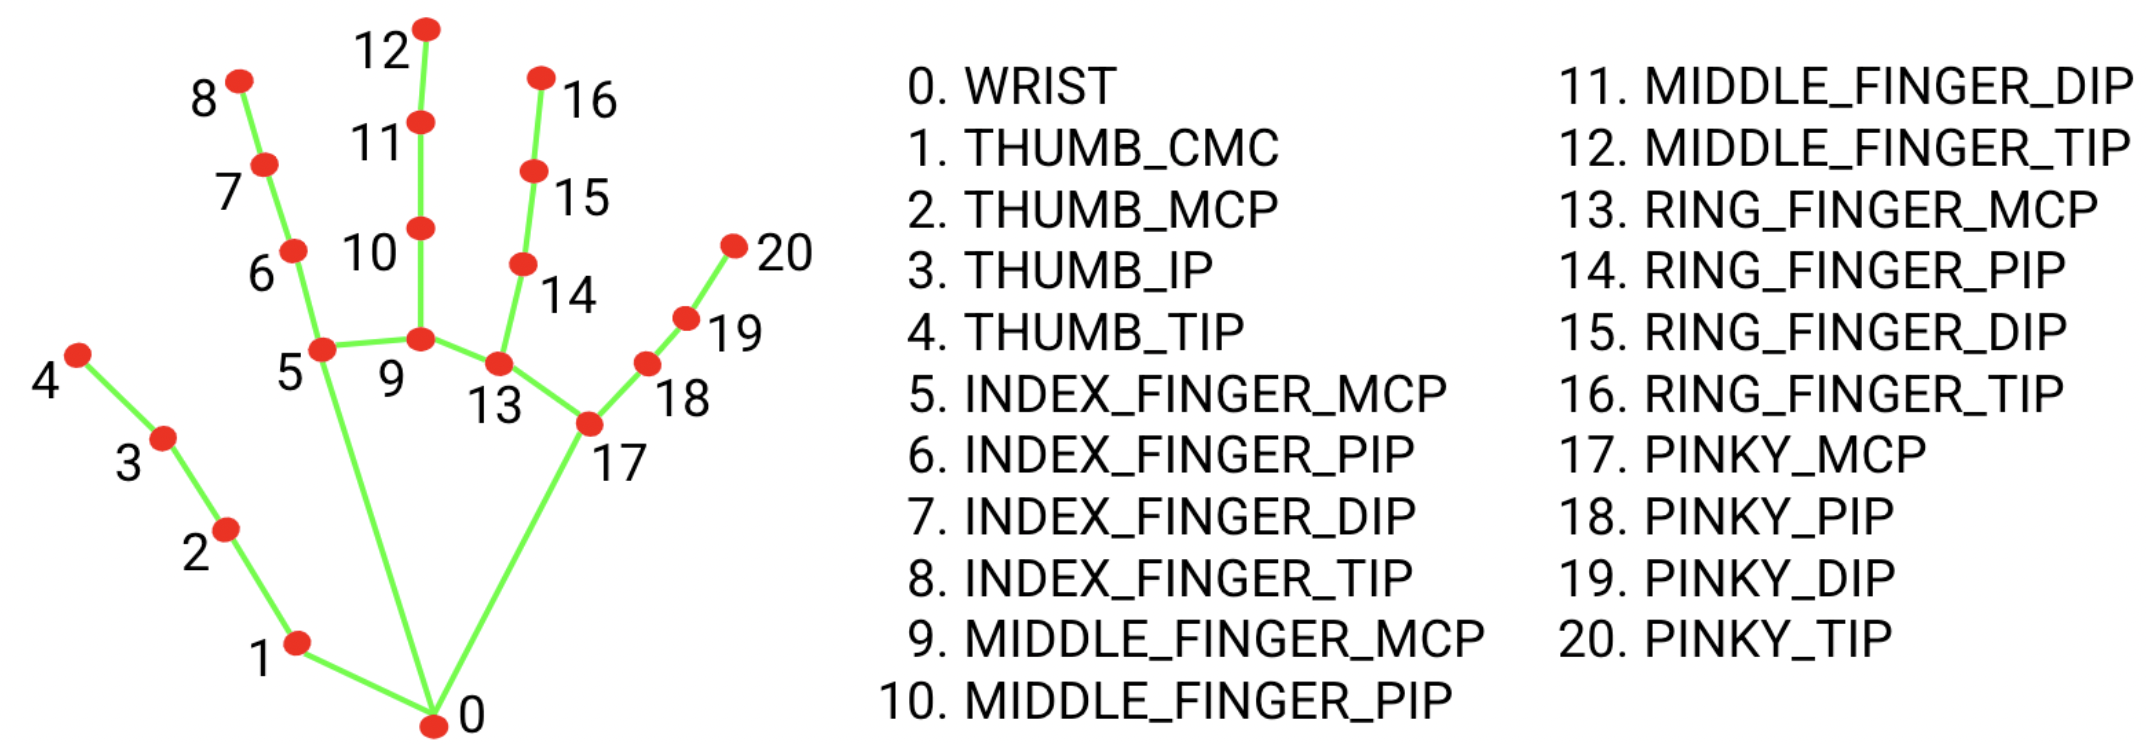
\includegraphics[width=0.8\textwidth]{Figure/hand-landmarks.png}
        \caption{MediaPipe Hand Landmark}
        \label{fig:mediapipe_hand_landmark}
    \end{figure}
    
Dalam desain sistem, tahap pertama adalah deteksi tangan menggunakan MediaPipe untuk mengenali tangan dan landmarknya secara akurat. Selanjutnya, posisi landmark tangan dianalisis untuk mengidentifikasi simbol angka ('0' hingga '5') berdasarkan aturan tertentu. Sistem juga mencakup pilihan operasi matematika, di mana antarmuka menampilkan menu operasi seperti penjumlahan, pengurangan, perkalian, dan pembagian, yang dapat dipilih menggunakan posisi jari telunjuk. Hasil deteksi angka dari kedua tangan dan operasi yang dipilih diintegrasikan untuk melakukan perhitungan, dengan hasil akhirnya ditampilkan langsung di layar secara interaktif \cite{Google2024}.
    
\section{Penjelasan Kode Program}
    \subsection{Import Library}
    Library yang diperlukan dalam program ini diantaranya cv2, mediapipe, dan numpy. 

    \begin{lstlisting}[language=Python, caption=Library yang Digunakan]
    
    import cv2
    import mediapipe as mp
    import numpy as np
    import pygame
    \end{lstlisting}
    Penjelasan:
    \begin{itemize}
    \item cv2 (OpenCV): Digunakan untuk memproses citra/video secara real-time, termasuk menangkap gambar dari webcam dan menampilkan hasil.
    \item mediapipe: Library dari Google untuk deteksi landmark tangan yang mendukung pengenalan gesture.
    \item numpy: Library untuk manipulasi array, meskipun dalam kode ini tidak digunakan secara eksplisit.
    \item pygame: Dalam hal ini, pygame digunakan untuk merender efek suara dengan method mixer.Sound()
    \end{itemize}

    \subsection{Memuat File Audio}
    \begin{lstlisting}[language=Python, caption=Memuat File Audio]
        
    sound_click = pygame.mixer.Sound("sfx/click.mp3")
    sound_success = pygame.mixer.Sound("sfx/succes.mp3")
    sound_error = pygame.mixer.Sound("sfx/error.mp3")
    \end{lstlisting}
    Penjelasan:
    \begin{itemize}
        \item $sound\_click$: Suara untuk klik operasi.
        \item $sound\_success$: Suara untuk hasil kalkulasi.
        \item $sound\_error$: Suara untuk kesalahan (misalnya, pembagian dengan nol).
    \end{itemize}

    \subsection{Inisialisasi MediaPipe}
    \begin{lstlisting}[language=Python, caption=Inisialisasi Mediapipe]
    
    mp_hands = mp.solutions.hands
    hands = mp_hands.Hands(min_detection_confidence=0.7, min_tracking_confidence=0.5)
    mp_drawing = mp.solutions.drawing_utils
    \end{lstlisting}
    \begin{itemize}
        \item mp.solutions.hands: Komponen MediaPipe untuk deteksi tangan.
        \item Hands: Menginisialisasi model deteksi tangan dengan confidence untuk deteksi dan pelacakan (0.7 dan 0.5 secara default).
        \item mp\_drawing: Komponen untuk menggambar landmark tangan pada frame yang diproses.
    \end{itemize}

    \subsection{Variabel Global}
    \begin{lstlisting}[language=Python, caption=Variabel Global]
    
    left_hand_signs_detected = []
    right_hand_signs_detected = []
    active_operation = None
    operation_processed = False
    last_result = None 
    operations = {"+": "Tambah", "-": "Kurang", "*": "Kali", "/": "Bagi"}
    selected = None
    last_selected = None
    \end{lstlisting}
    Penjelasan:
    \begin{itemize}
        \item $left\_hand\_signs\_detected$ dan $right\_hand\_signs\_detected$: Menyimpan angka yang terdeteksi dari masing-masing tangan.
        \item $active\_operation$: Menyimpan operasi matematika yang dipilih (misalnya, "+", "-", "*", "/").
        \item $operation\_processed$: Flag untuk memastikan operasi hanya diproses sekali.
        \item $last\_result$: Variabel untuk menyimpan hasil terakhir
        \item $operations$: Dictionary untuk mencocokkan simbol operasi dengan deskripsinya.
        \item $selected$ dan $last\_selected$: Variabel untuk menyimpan operasi matematika yang dipilih supaya efek suara tidak dimainkan berkali-kali.
    \end{itemize}

    \subsection{Variabel Kelola Waktu Jeda}
    \begin{lstlisting}[language=Python, caption=Variabel Kelola Waktu Jeda]
        
    last_sound_time = 0
    click_delay = 1
    \end{lstlisting}
    \begin{itemize}
        \item $last\_sound\_time$: Waktu terakhir suara diputar.
        \item $click\_delay$: Waktu jeda antara suara klik.
    \end{itemize}

    \subsection{Fungsi play\_sound\_with\_delay}
    \begin{lstlisting}[language=Python, caption=Fungsi memainkan suara dengan jeda]

    global last_sound_time
    current_time = time.time()
    if current_time - last_sound_time >= delay:
        sound.play()
        last_sound_time = current_time
    \end{lstlisting}
    Penjelasan:
    \begin{itemize}
        \item Fungsi ini memainkan suara dengan jeda tertentu.
        \item sound: Objek suara yang akan diputar.
        \item delay: Waktu jeda antara pemutaran suara.
        \item Variabel global last\_sound\_time digunakan untuk menyimpan waktu terakhir suara diputar.
        \item Fungsi ini memeriksa apakah waktu sekarang sudah melewati waktu jeda sebelum memainkan suara.
        \item Jika sudah melewati waktu jeda, suara diputar dan last\_sound\_time diperbarui.
    \end{itemize}

    \subsection{Fungsi detect\_hand\_sign}
    \begin{lstlisting}[language=Python, caption=Fungsi Mendeteksi Landmark Tangan]
    
    def detect_hand_sign(landmarks, handedness):

        # Untuk tangan kanan (handedness == 'Right')
        if handedness == "Right":
            # Mengecek apakah tangan membentuk simbol 'nol'
            if (landmarks[4].x > landmarks[3].x and landmarks[8].y > landmarks[6].y and landmarks[12].y > landmarks[10].y and landmarks[16].y > landmarks[14].y and landmarks[20].y > landmarks[18].y):
                return '0'
            # Mengecek apakah tangan membentuk simbol 'satu'
            if (landmarks[4].x > landmarks[3].x and landmarks[8].y < landmarks[6].y and landmarks[12].y > landmarks[10].y and landmarks[16].y > landmarks[14].y and landmarks[20].y > landmarks[18].y):
                return '1'
            # Mengecek apakah tangan membentuk simbol 'dua'
            if (landmarks[4].x > landmarks[3].x and landmarks[8].y < landmarks[6].y and landmarks[12].y < landmarks[10].y and landmarks[16].y > landmarks[14].y and landmarks[20].y > landmarks[18].y):
                return '2'
            # Mengecek apakah tangan membentuk simbol 'tiga'
            if (landmarks[4].x > landmarks[3].x and landmarks[8].y < landmarks[6].y and landmarks[12].y < landmarks[10].y and landmarks[16].y < landmarks[14].y and landmarks[20].y > landmarks[18].y):
                return '3'
            # Mengecek apakah tangan membentuk simbol 'empat'
            if (landmarks[4].x > landmarks[3].x and landmarks[8].y < landmarks[6].y and landmarks[12].y < landmarks[10].y and landmarks[16].y < landmarks[14].y and landmarks[20].y < landmarks[18].y):
                return '4'
            # Mengecek apakah tangan membentuk simbol 'lima'
            if (landmarks[4].x <= landmarks[3].x and landmarks[8].y < landmarks[6].y and landmarks[12].y < landmarks[10].y and landmarks[16].y < landmarks[14].y and landmarks[20].y < landmarks[18].y):
                return '5'
            
        # Untuk tangan kiri (handedness == 'Left')
        if handedness == "Left":
            # Mengecek apakah tangan membentuk simbol 'nol'
            if (landmarks[4].x <= landmarks[3].x and landmarks[8].y > landmarks[6].y and landmarks[12].y > landmarks[10].y and landmarks[16].y > landmarks[14].y and landmarks[20].y > landmarks[18].y):
                return '0'
            # Mengecek apakah tangan membentuk simbol 'satu'
            if (landmarks[4].x <= landmarks[3].x and landmarks[8].y < landmarks[6].y and landmarks[12].y > landmarks[10].y and landmarks[16].y > landmarks[14].y and landmarks[20].y > landmarks[18].y):
                return '1'
            # Mengecek apakah tangan membentuk simbol 'dua'
            if (landmarks[4].x <= landmarks[3].x and landmarks[8].y < landmarks[6].y and landmarks[12].y < landmarks[10].y and landmarks[16].y > landmarks[14].y and landmarks[20].y > landmarks[18].y):
                return '2'
            # Mengecek apakah tangan membentuk simbol 'tiga'
            if (landmarks[4].x <= landmarks[3].x and landmarks[8].y < landmarks[6].y and landmarks[12].y < landmarks[10].y and landmarks[16].y < landmarks[14].y and landmarks[20].y > landmarks[18].y):
                return '3'
            # Mengecek apakah tangan membentuk simbol 'empat'
            if (landmarks[4].x <= landmarks[3].x and landmarks[8].y < landmarks[6].y and landmarks[12].y < landmarks[10].y and landmarks[16].y < landmarks[14].y and landmarks[20].y < landmarks[18].y):
                return '4'
            # Mengecek apakah tangan membentuk simbol 'lima'
            if (landmarks[4].x > landmarks[3].x and landmarks[8].y < landmarks[6].y and landmarks[12].y < landmarks[10].y and landmarks[16].y < landmarks[14].y and landmarks[20].y < landmarks[18].y):
                return '5'
        
    return None
    \end{lstlisting}
    Penjelasan:
    \begin{itemize}
    \item Fungsi ini mendeteksi simbol angka ('0'-'5') berdasarkan posisi landmark tangan.
    \item Parameter:
        \item landmarks: Koordinat landmark tangan yang dihasilkan oleh MediaPipe.
        \item handedness: Menentukan apakah tangan adalah kiri atau kanan.
    \item Logika Deteksi:
        \item  Setiap angka diwakili oleh posisi spesifik jari:
            \item Jari tertutup: Landmark y dari ruas atas jari lebih besar dari landmark y ruas bawah.
            \item Jari terbuka: Landmark y dari ruas atas lebih kecil dari landmark y ruas bawah.
    \item Fungsi mengembalikan angka ('0'-'5') jika simbol dikenali atau None jika tidak ada simbol yang valid.
    \end{itemize}

    \subsection{Fungsi detect\_operation}
    \begin{lstlisting}[language=Python, caption=Fungsi Mendeteksi Operasi Aktif]
    
    def detect_operation(x, y):
        global selected, last_selected
        selected = False
        for i, (symbol, label) in enumerate(operations.items()):
            if 10 <= x <= 130 and 50 + i * 60 <= y <= 90 + i * 60:
                if last_selected != symbol:
                    play_sound_with_delay(sound_click, click_delay)
                    last_selected = symbol
        return symbol
        last_selected = None
        return None
    \end{lstlisting}
    Penjelasan:
    \begin{itemize}
        \item Fungsi mendeteksi operasi matematika yang dipilih berdasarkan posisi jari telunjuk (koordinat x, y).
        \item Parameter x, y merupakan posisi jari telunjuk pada layar dalam piksel.
        \item Loogika deteksinya jika jari telunjuk berada di dalam kotak menu operasi (dengan koordinat tetap di layar), simbol operasi dikembalikan
    \end{itemize}

    \subsection{Fungsi calculate\_result}
    \begin{lstlisting}[language=Python, caption=Fungsi Perhitungan]
    
    def calculate_result(left, right, operation):
        global operation_processed, last_result
        if operation == "*":
            display_op = "x"
        else:
            display_op = operation
        
        if operation_processed:
            return last_result, display_op
        
        left = int(left)
        right = int(right)
        result = None
        if operation == "+":
            result = left + right
        elif operation == "-":
            result = left - right
        elif operation == "*" and right != 0:
            result = left * right
        elif operation == "/" and right != 0:
            result = left / right
        else:
            result = "Error"
            sound_error.play()
        if result != "Error":
            sound_success.play()

        operation_processed = True
        last_result = result
        return result, display_op
    \end{lstlisting}
    Penjelasan:
    \begin{itemize}
        \item Fungsi menghitung hasil berdasarkan angka dari tangan kiri dan kanan serta operasi yang dipilih.
        \item Parameter left (angka dari tangan kiri), right (angka dari tangan kanan), dan operation (perasi matematika yang dipilih).
        \item Logika perhitungannya yaitu melakukan perhitungan sesuai dengan simbol operasi dan mengembalikan hasil operasi atau pesan "Error" jika operasi tidak valid (misalnya pembagian oleh nol).
    \end{itemize}

    \subsection{Fungsi draw\_text\_with\_stroke}
    \begin{lstlisting}[language=Python, caption=Fungsi Menulis Teks dengan Stroke]

    x, y = position
    for dx, dy in [(-1, -1), (-1, 1), (1, -1), (1, 1)]:
        cv2.putText(img, text, (x + dx, y + dy), font, scale, color_stroke, thickness_stroke)

    cv2.putText(img, text, (x, y), font, scale, color_text, thickness_text)
    \end{lstlisting}
    Penjelasan:
    \begin{itemize}
        \item Fungsi ini digunakan untuk menulis teks dengan efek stroke pada gambar.
        \item Parameter:
            \item img: Gambar yang akan ditulis.
            \item text: Teks yang akan ditulis.
            \item position: Koordinat (x, y) untuk posisi teks.
            \item font: Font teks.
            \item scale: Skala teks.
            \item color\_stroke: Warna stroke teks.
            \item thickness\_stroke: Ketebalan stroke.
            \item color\_text: Warna teks.
            \item thickness\_text: Ketebalan teks.
            \item Fungsi ini menulis teks dengan stroke menggunakan 4 arah (atas, bawah, kiri, kanan) untuk memberikan efek bayangan pada teks. 
            \item Kemudian, teks utama ditulis di tengah dengan warna teks yang berbeda.
            \item Ini memberikan efek teks dengan stroke yang lebih menarik dan mudah dibaca.
    \end{itemize}

    \subsection{Fungsi main}
    
    Membuka webcam untuk menangkap video real-time.
    \begin{lstlisting}[language=Python, caption=Membuka Webcam]
    
    cap = cv2.VideoCapture(0)
    \end{lstlisting}

    Membaca frame dari webcam dan memprosesnya secara terus-menerus hingga tombol keluar ditekan.
    \begin{lstlisting}[language=Python, caption=Membaca Frame]
    
    while cap.isOpened():
        ret, frame = cap.read()
        ...
    \end{lstlisting}
    
    Membalik frame secara horizontal untuk memberikan tampilan seperti cermin.
    \begin{lstlisting}[language=Python, caption=Mirror Camera]
    
    frame = cv2.flip(frame, 1)
    \end{lstlisting}

    Mengubah frame dari BGR ke RGB (MediaPipe memerlukan format RGB) dan menjalankan deteksi tangan dengan hands.process(frame\_rgb).
    \begin{lstlisting}[language=Python, caption=Konversi ke RGB]
    
    frame_rgb = cv2.cvtColor(frame, cv2.COLOR_BGR2RGB)
    results = hands.process(frame_rgb)
    \end{lstlisting}

    Landmark tangan digambar pada frame menggunakan MediaPipe Drawing Utilities
    \begin{lstlisting}[language=Python, caption=Menggambar Landmark]
    
    for idx, hand_landmarks in enumerate(results.multi_hand_landmarks):
        mp_drawing.draw_landmarks(frame, hand_landmarks, mp_hands.HAND_CONNECTIONS)
        ...
    \end{lstlisting}

    detect\_hand\_sign digunakan untuk mendeteksi angka pada tangan kiri dan kanan.
    \begin{lstlisting}[language=Python, caption=Proses Deteksi Nilai Tangan]

    hand_sign = detect_hand_sign(hand_landmarks.landmark, handedness)
    ...
    \end{lstlisting}

    Posisi jari telunjuk (landmark ke-8) digunakan untuk mendeteksi operasi yang dipilih dari menu.
    \begin{lstlisting}[language=Python, caption=Pemilihan Operasi]
    
    selected_operation = detect_operation(x, y)
    \end{lstlisting}

    Jika simbol tangan dan operasi terdeteksi, hasil perhitungan dihitung menggunakan calculate\_result.
    \begin{lstlisting}[language=Python, caption=Proses Kalkulasi]
    
    if active_operation and left_hand_signs_detected and right_hand_signs_detected:
        result, display_op = calculate_result(left_hand_signs_detected[0], right_hand_signs_detected[0], active_operation)
    \end{lstlisting}

    Menampilkan hasil perhitungan, angka dari masing-masing tangan, dan operasi yang aktif pada layar
    \begin{lstlisting}[language=Python, caption==Output Hasil Perhitungan,]
    
    draw_text_with_stroke(frame, f"Hasil: {result}", (200, 100), ...)
    \end{lstlisting}

    Program keluar dari loop jika tombol "q" ditekan.
    \begin{lstlisting}[language=Python, caption=Escape Program]
    
    if cv2.waitKey(1) & 0xFF == ord("q"):
        break
    \end{lstlisting}
    \subsection{Eksekusi Program}
    Program akan memulai eksekusi dari fungsi main.
    \begin{lstlisting}[language=Python, caption=Eksekusi Program]
    
    if __name__ == "__main__":
        main()
    \end{lstlisting}

\newpage
\section{Hasil dan Pembahasan}
    \subsection{Hasil}

    Program berhasil mendeteksi simbol angka ('0'-'5') dari pose tangan dan operasi matematika yang dipilih menggunakan jari telunjuk. Hasil perhitungan ditampilkan secara real-time di layar berdasarkan input dari gesture tangan. Program juga menyertakan efek suara untuk setiap interaksi, seperti memilih operasi matematika, hasil perhitungan, dan kesalahan (misalnya, pembagian dengan nol). Berikut adalah contoh hasil program saat digunakan:
    \begin{figure}[H]
        \centering
        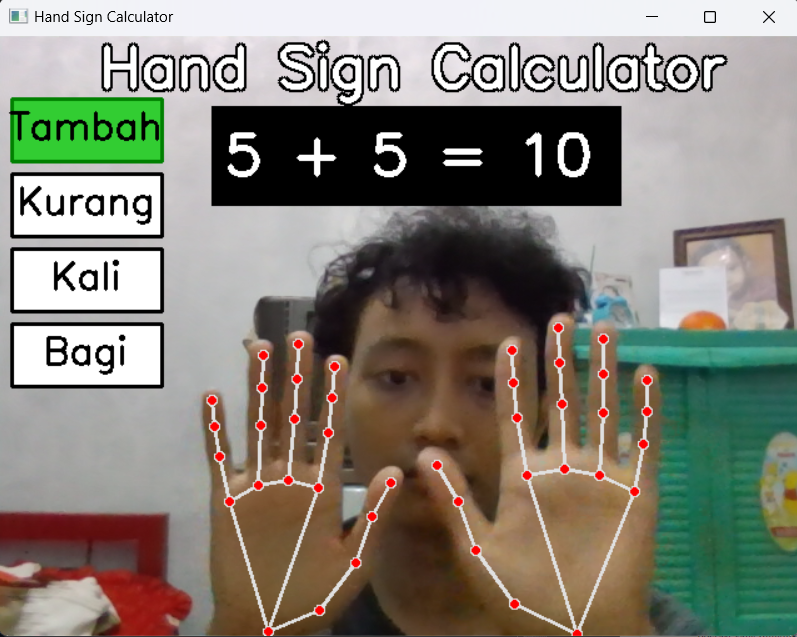
\includegraphics[width=0.5\textwidth]{Figure/hand-sign-calculator.png}
        \caption{Hasil Run Program}
        \label{fig:hand_sign_calculator}
    \end{figure}
    \begin{figure}[H]
        \centering
        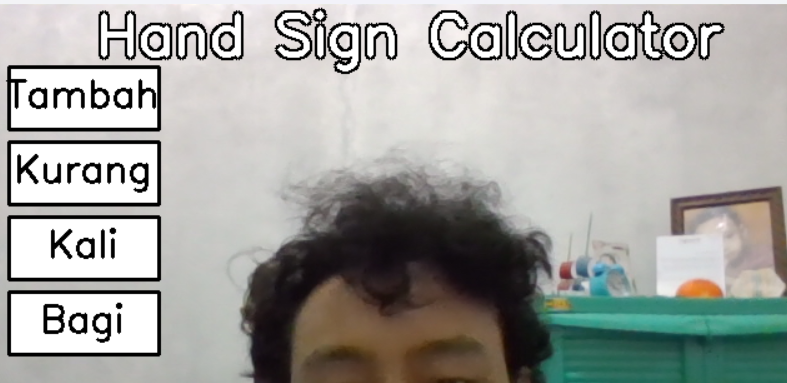
\includegraphics[width=0.8\textwidth]{Figure/menu_button.png}
        \caption{Antarmuka Menu Operasi}
        \label{fig:menu_button}
    \end{figure}
    Terdapat menu operasi matematika yang dapat dipilih dengan menunjuk jari telunjuk ke simbol operasi yang diinginkan. Hasil perhitungan ditampilkan di layar berdasarkan input dari gesture tangan. Program juga menyertakan efek suara untuk meningkatkan interaktivitas dan memberikan umpan balik kepada pengguna. Ada 4 tombol operasi matematika yang dapat dipilih, yaitu penjumlahan, pengurangan, perkalian, dan pembagian. Tombol operasi matematika dapat dipilih dengan menunjuk jari telunjuk ke simbol operasi yang diinginkan. Hasil perhitungan ditampilkan di layar berdasarkan input dari gesture tangan. Program juga menyertakan efek suara untuk meningkatkan interaktivitas dan memberikan umpan balik kepada pengguna.
    \begin{figure}[H]
        \centering
        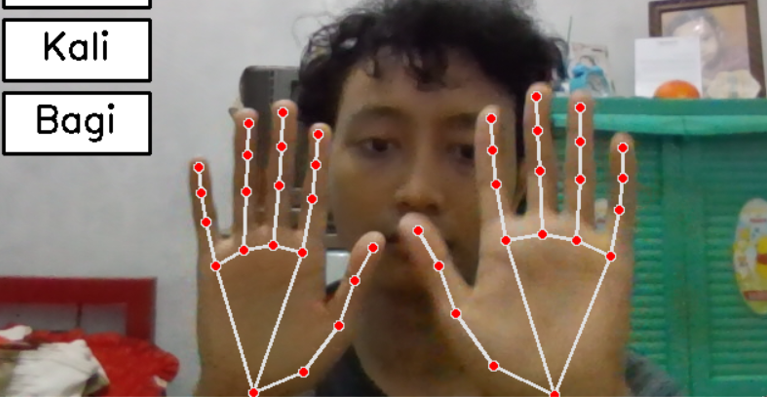
\includegraphics[width=0.8\textwidth]{Figure/number_detection.png}
        \caption{Deteksi Simbol Angka}
        \label{fig:number_detection}
    \end{figure}
    Program dapat mendeteksi simbol angka ('0'-'5') berdasarkan pose tangan yang dibentuk. Setiap simbol angka diwakili oleh posisi jari tertentu yang membentuk simbol tersebut. Hasil perhitungan ditampilkan secara real-time di layar berdasarkan input dari gesture tangan. Program juga menyertakan efek suara untuk meningkatkan interaktivitas dan memberikan umpan balik kepada pengguna.

    \subsection{Pembahasan}

    Implementasi MediaPipe dan OpenCV memungkinkan program untuk mendeteksi landmark tangan dan mengenali simbol angka dengan akurat. Logika deteksi simbol angka didasarkan pada posisi jari tertentu yang membentuk simbol tertentu. Pemilihan operasi matematika menggunakan posisi jari telunjuk yang menunjuk ke menu operasi. Hasil perhitungan ditampilkan secara real-time di layar berdasarkan input dari gesture tangan. Program juga menyertakan efek suara untuk meningkatkan interaktivitas dan memberikan umpan balik kepada pengguna. Namun, program masih memiliki beberapa kekurangan, seperti sensitivitas terhadap pencahayaan dan latar belakang, serta keterbatasan dalam mendeteksi simbol angka yang kompleks. Untuk pengembangan selanjutnya, dapat dilakukan peningkatan dalam deteksi landmark tangan, pengenalan simbol angka yang lebih kompleks, dan integrasi dengan fitur lain seperti pengenalan gesture tambahan dan antarmuka pengguna yang lebih interaktif.

\newpage
\section{Cara Instalasi dan Penggunaan}
    \subsection{Cara Instalasi}
    Clone repository ini.
    \begin{lstlisting}[language=Python, caption=Clone Repository]
    
    git clone https://github.com/redywi/hand-sign-calculator.git  
    cd hand-sign-calculator  
    \end{lstlisting}
    Install depencencies.
    \begin{lstlisting}[language=Python, caption=Pemasangan Dependencies]
    
    pip install -r requirements.txt   
    \end{lstlisting}

    \subsection{Penggunaan}
    Jalankan program.
    \begin{lstlisting}[language=Python, caption=Jalankan Program]

    python main.py  
    \end{lstlisting}
    Arahkan tangan ke kamera dan gunakan simbol berikut:
    \begin{itemize}
        \item Tangan kiri untuk angka pertama.
        \item Tangan kanan untuk angka kedua.
        \item Perlu diingat telapak tangan harus menghadap ke depan.
        \item Pilih operasi matematika dengan jari telunjuk.
    \end{itemize}
    Hasil perhitungan akan ditampilkan secara real-time di layar.
    
\newpage
\bibliographystyle{IEEEtran}
\bibliography{Referensi}
\end{document}